\section{Statistical Analysis}

\textbf{Data Collection}

Important:
\begin{itemize}
    \item Choose representative sample
    \item Form hypthesis to make asssumptions testable
    \item collect data to test Hypothesis
    \item collect all avaiable data (better too much)
\end{itemize}
\textit{Population vs Sample}


\begin{center}
	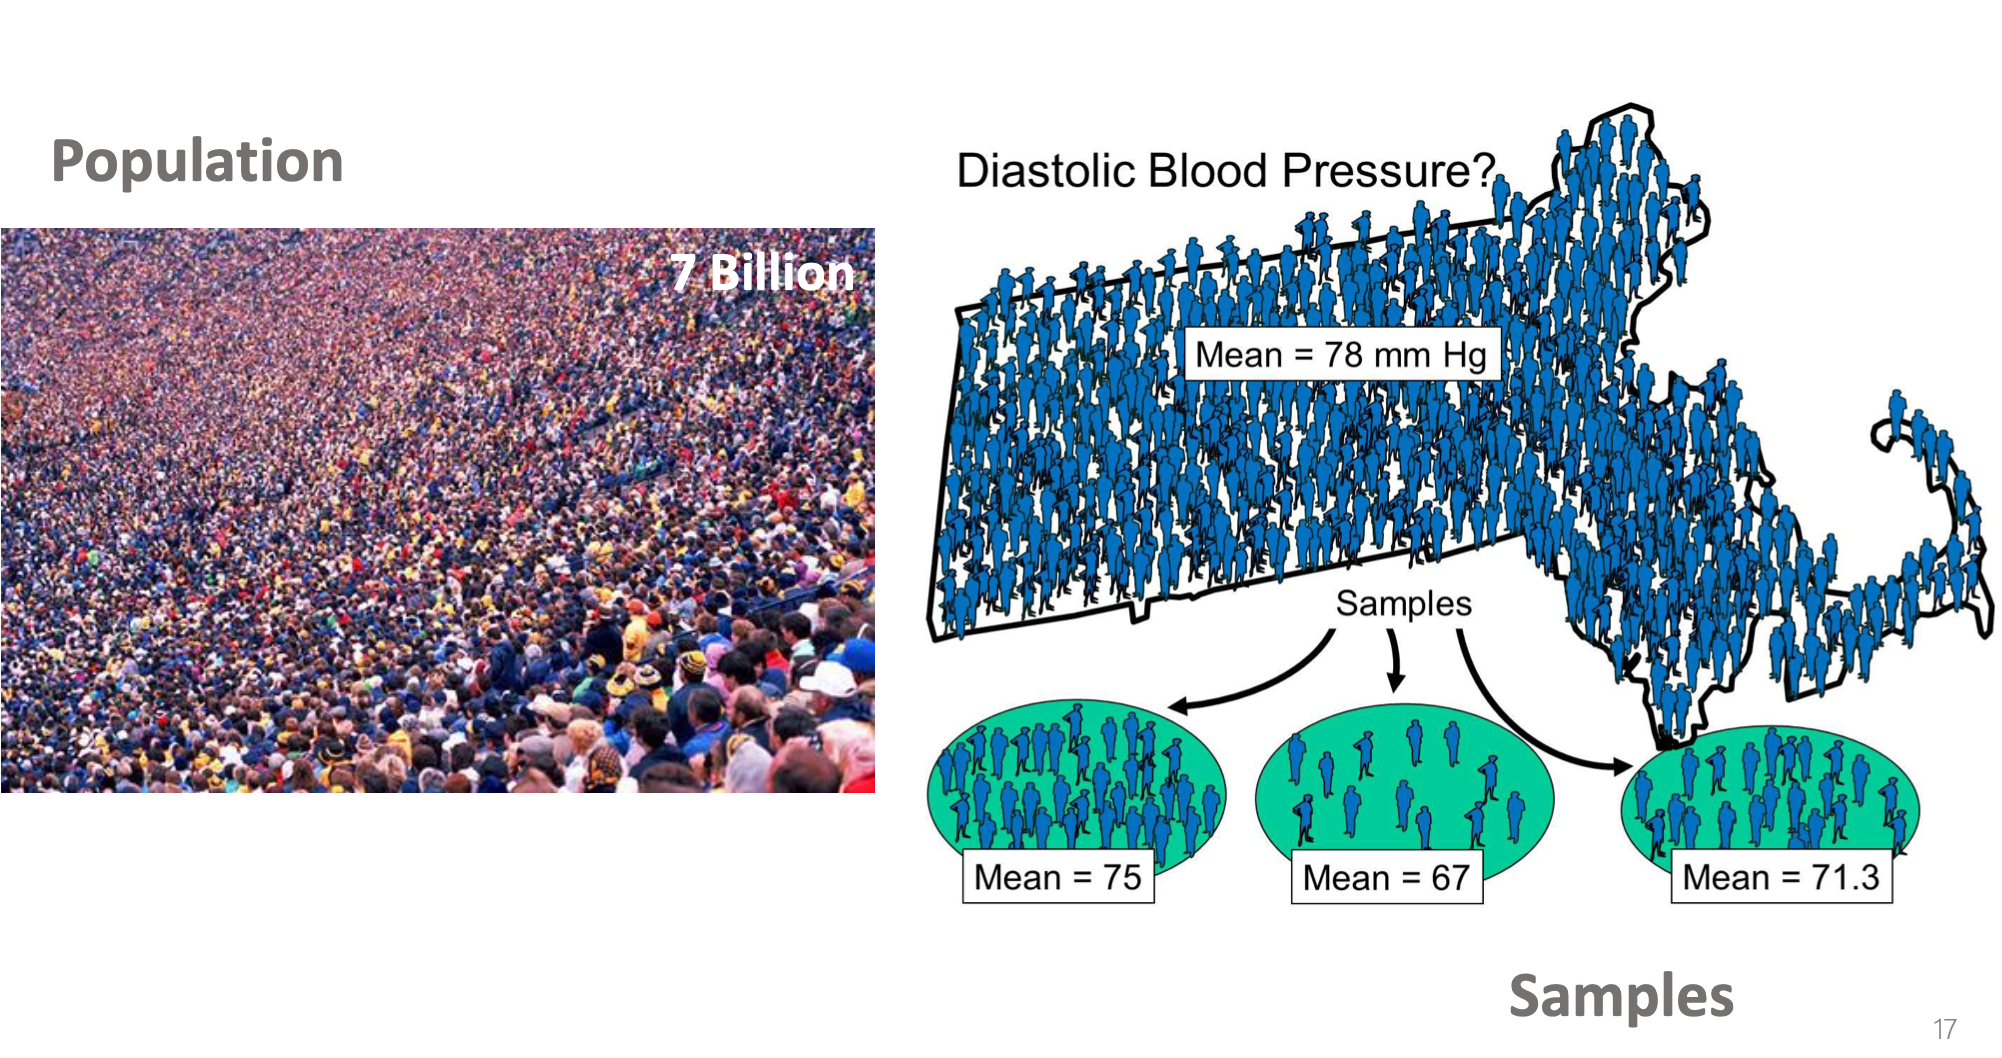
\includegraphics[width=\linewidth]{population_sample.png}
\end{center}


\textit{Generalizability} \smallskip

Results should be valid for all people. Participants should be representative of population. Look at relevant factors, such as Age, Gender, Occupation. \medskip

\textit{Hypothesis testing}  \smallskip

Effect size is difference in the means of $H_A$ and $H_0$. It is unknown a-priori and hence we don't know how to show the threshold for acceptance. 
Therefore instead of showing $H_A$ is true, we show that the obtained data is incompatible with $H_0$. \bigskip

\textbf{Descriptive statistics and validation}  \smallskip

How should data be validated? \medskip

\textit{Mean}  \smallskip

Least distance to all other data points. Good representation of data points piled together. Bad representation if some data points are extreme values (outliers).
Doesn't make sense if we divide through categorical or ordinal data. \medskip

\textit{Median}  \smallskip

is robust against outliers. The number at the middle of the ordered data points. Natural choice to represent ordinal data. \medskip

\textit{Distribution} \smallskip


\begin{center}
	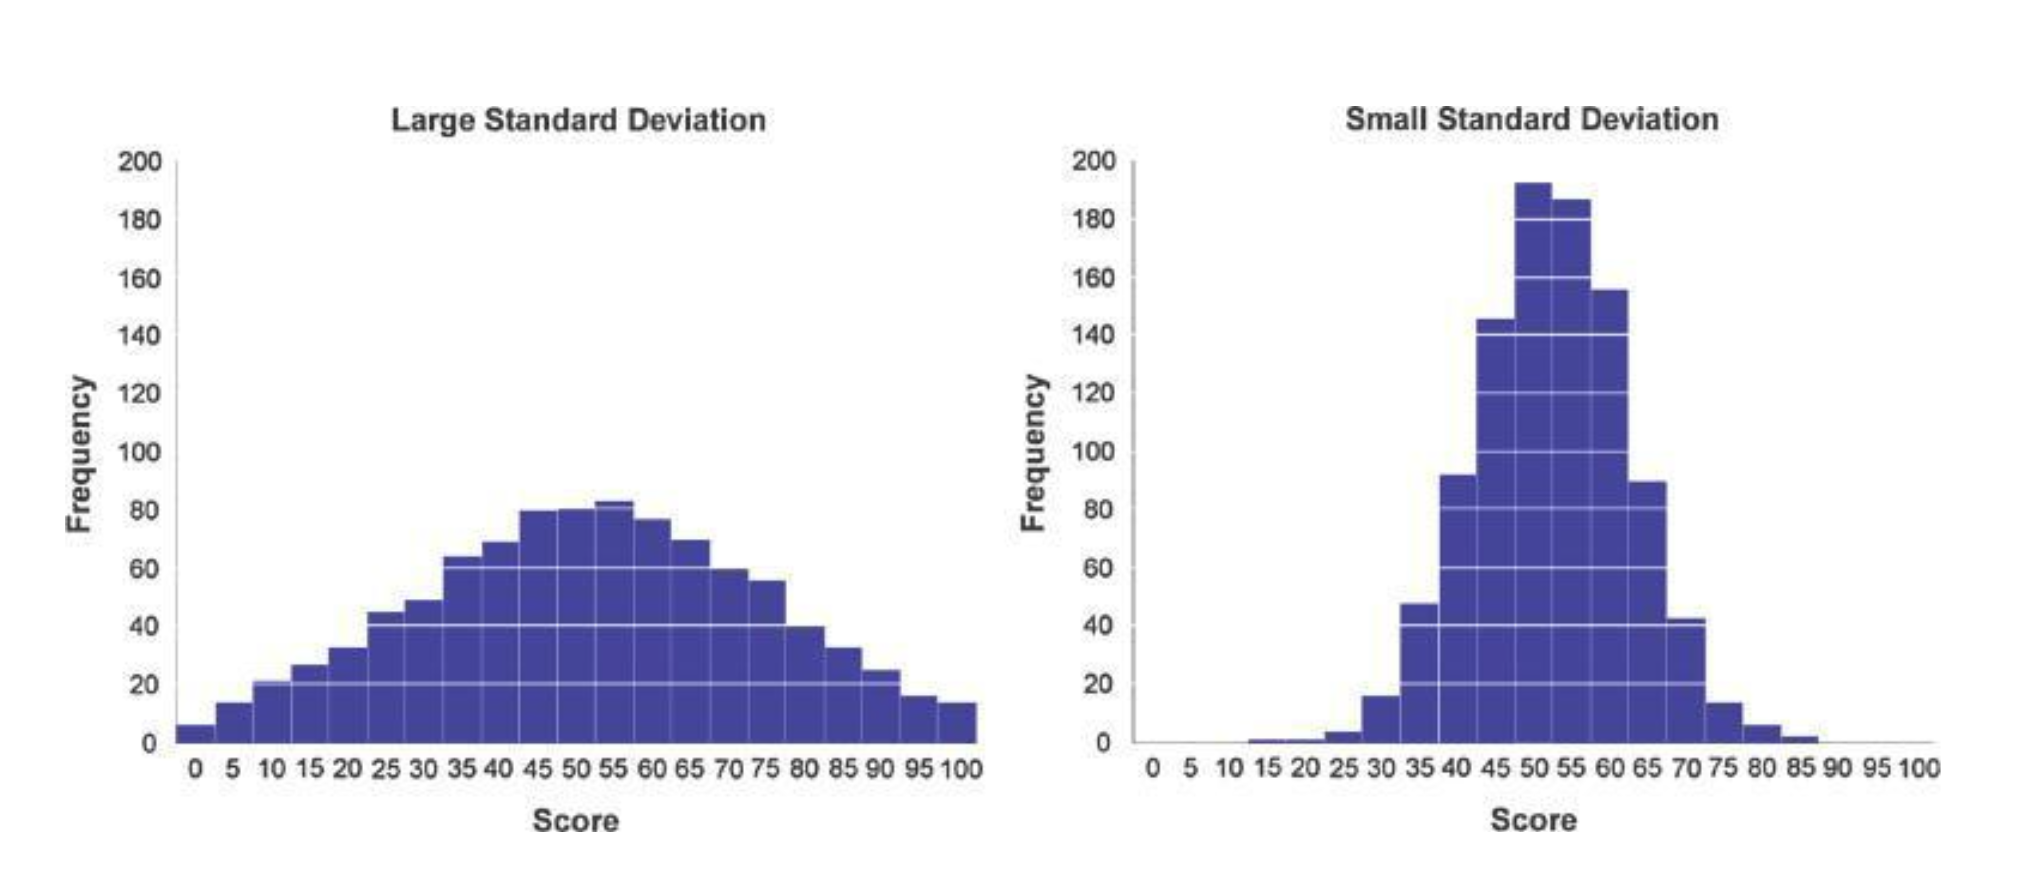
\includegraphics[width=\linewidth]{standard_deviation.png}
\end{center}


\textit{Confidence Interval (CI)} \smallskip

Interval in which we are very sure that our true values lie in. We mostly choose 95 percent of values to lie within this interval if often replicated. 
Confidence interval of mean difference (two samples) \medskip

 \textbf{Analysis} \smallskip

 Bayesian quantitative approach no covered in this course, also not qualitative analysis methods. \medskip

\textbf{Frequentist Approaches} \smallskip

\textit{Hypothesis testing} \smallskip

We assume $H_0$ to be true. The lower our p-value the less likely that $H_0$ is true and $H_A$ is true. P-value indicated how compatible the data to which hypothesis is. \medskip

\textit{P-Value} \smallskip

P-value is probability of observed data if $H_0$ were true.

\begin{center}
	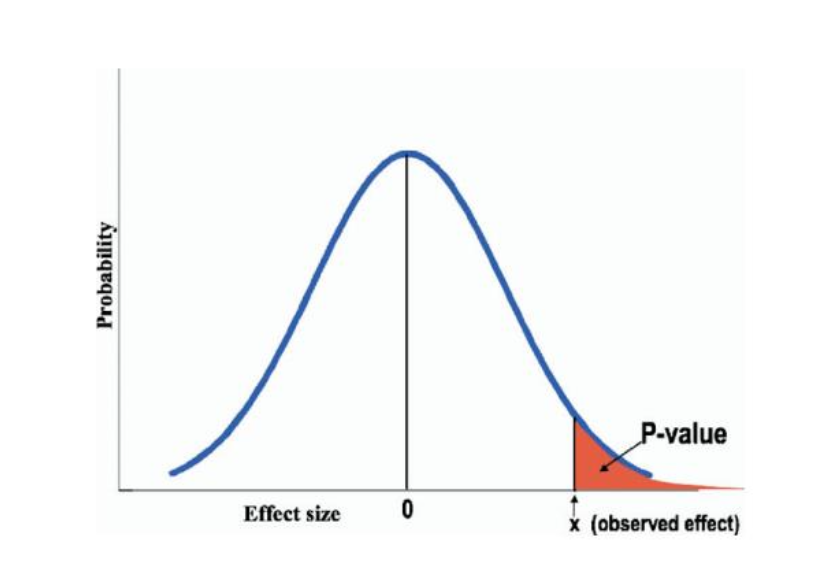
\includegraphics[width=\linewidth]{p_value.png}
\end{center}


\textit{Alpha-Level} \smallskip

Threshold to determine if p-value is lowe enough. Usually $\alpha = 0.05$. In medicine even lower.
If p-vlue is larger than $\alpha$ this does not mean that $H_0$ is true! \medskip


\begin{center}
	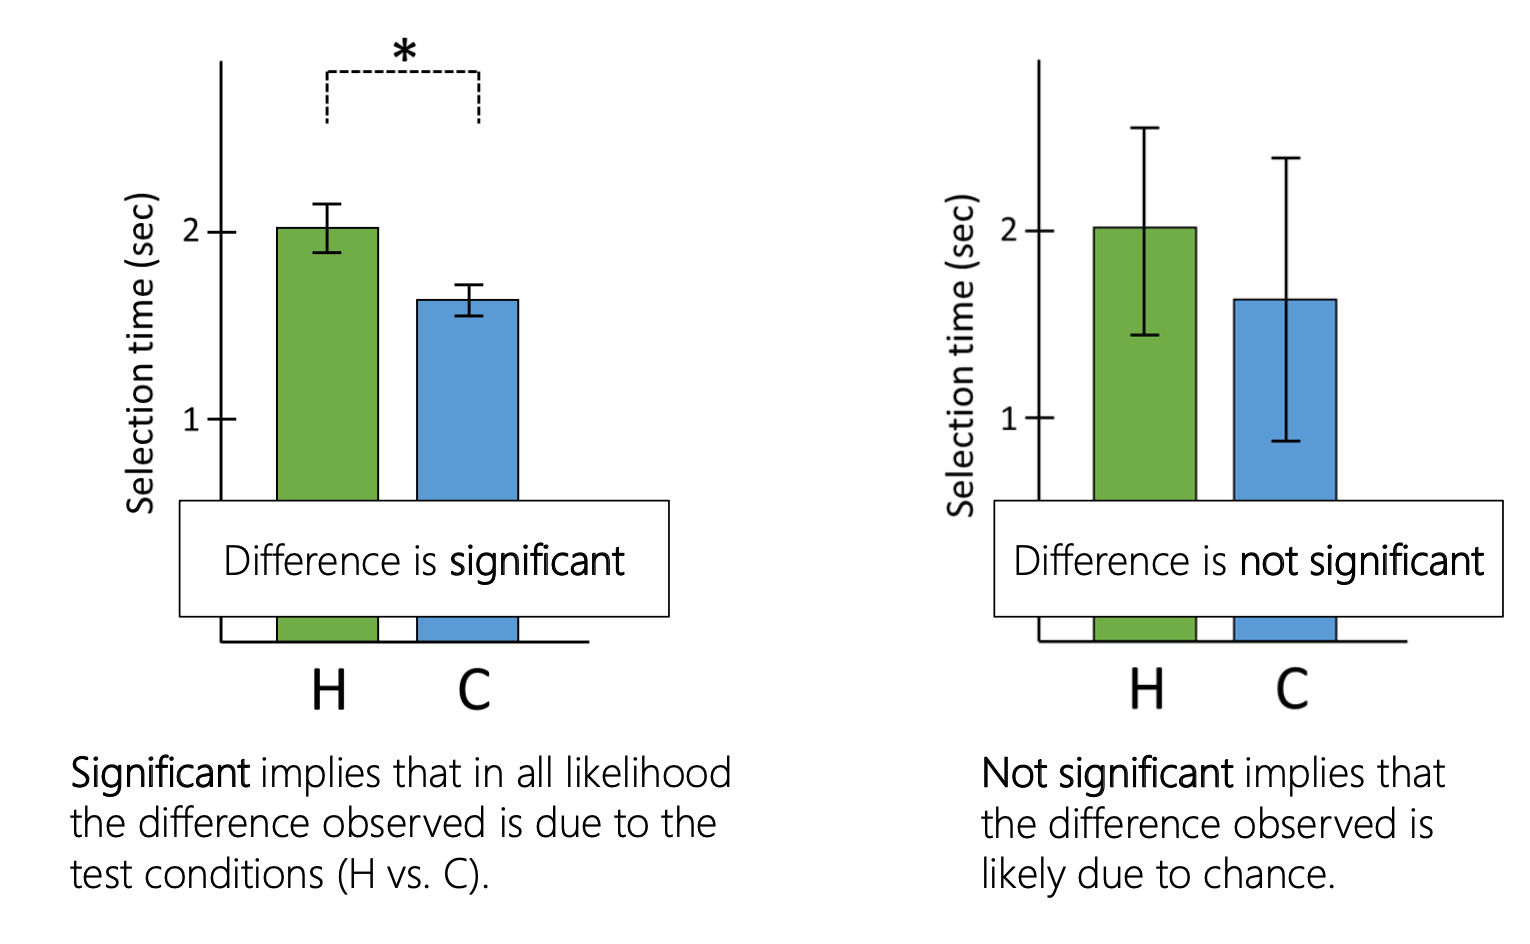
\includegraphics[width=\linewidth]{differences_mean.png}
\end{center}



\textit{Errors} \smallskip

Type I error: Effect was found, but no effect in reality (False-Positive).

Type II error: No effect was found, but effect exists in reality (False-Negative). \medskip

\textit{Degrees of Freedom} \smallskip

Number of values that are free to cary. Number of observations ($n$) minus the number of parameter estimates. For one-sample t-test: $$v = n-1$$. \medskip

\textit{Independent vs dependent samples} \smallskip

Independent: One subject only exposed to one condition (use different subjects for differen conditions). Also referred to as Independent measures or means. 

Dependent: Same subject exposed to all conditions (Within subject design). Also referred to as matched pairs or paired samples. \medskip


\textit{Parametrix vs. non-parametric tests} \smallskip

Non-parametric do not assume specific distribution. Assume equal spread of group samples. Less statistical power. Type II error more likely. 

Examples: Chi-Square, Mann Whitnes, Wilcoxons signed rank test, Kruskal Wallis, Friedman \medskip

Parametric tests assume gaussian distribution and homoscedasticity (equal variances). More power!

Examples: one-sample t-test, two-sample t-test, paired-sample t-test, one-way/factorial ANOVA, repeated measured ANOVA. \medskip

\textit{A/B Testing} \smallskip

Common example as in our case: Change one categorical independent variable with two levels (A and B) and measure one interval dependent variable.
In our case task execution time. \medskip

\textit{Independent t-test} \smallskip

Checks if two means are reliably different from each other. $ t = $(variance between groups) /(variance within groups).

Large t means different groups ($H_0$ refuted). \medskip

\textit{From t-value to significance} \smallskip

T-values lead us to our p-value over degrees of freedom in standardized tables. 
T-distribution depends on sample size (degrees of freedom). Its a distribution of t-values of a population where the null hypothesis is true. \medskip

\textit{ANOVA analysis of Variance} \smallskip

Use this if independent variable /factor has three or more levels. One-way ANOVA is used for data with one factor and multiple levels. 
Factorial ANOVA is used for data with multiple factors and levels. Does not tell us which levels are different. \medskip

\textit{Effect size} \smallskip

Statistical significance does not mean that the measured effect is meaningful. So we need a standardized effect size. We use Cohen's d, Pearson's correlation, odds ratio. 

Cohens' d is a standardized mean difference between the samples. Depends on the field. 

$$\text{Cohen's } d = \frac{\text{mean}(A) - \text{mean}(B)}{\text{mean}([\text{std}(A), \text{std}(B)])}$$

\textit{Power analysis} \smallskip

Compute min. number of participants to achieve desired effect. Can be calculated from 

\begin{itemize}
    \item prob. of finding an effect that is not there ($\alpha = 0.05$)
    \item prob. of finding an effect that is there ($1-\beta = 0.8$)
    \item the desired effect size (HCI d = 0.8)
  
\end{itemize}

\textit{Software for statistical analysis} \smallskip

\begin{multicols}{4}
    \begin{itemize}
        \item SPSS
        \item Python
        \item R
        \item etc. 
    \end{itemize}
\end{multicols}


\textbf{Reporting} \smallskip


\textit{Writing up the results} \smallskip

\begin{center}
	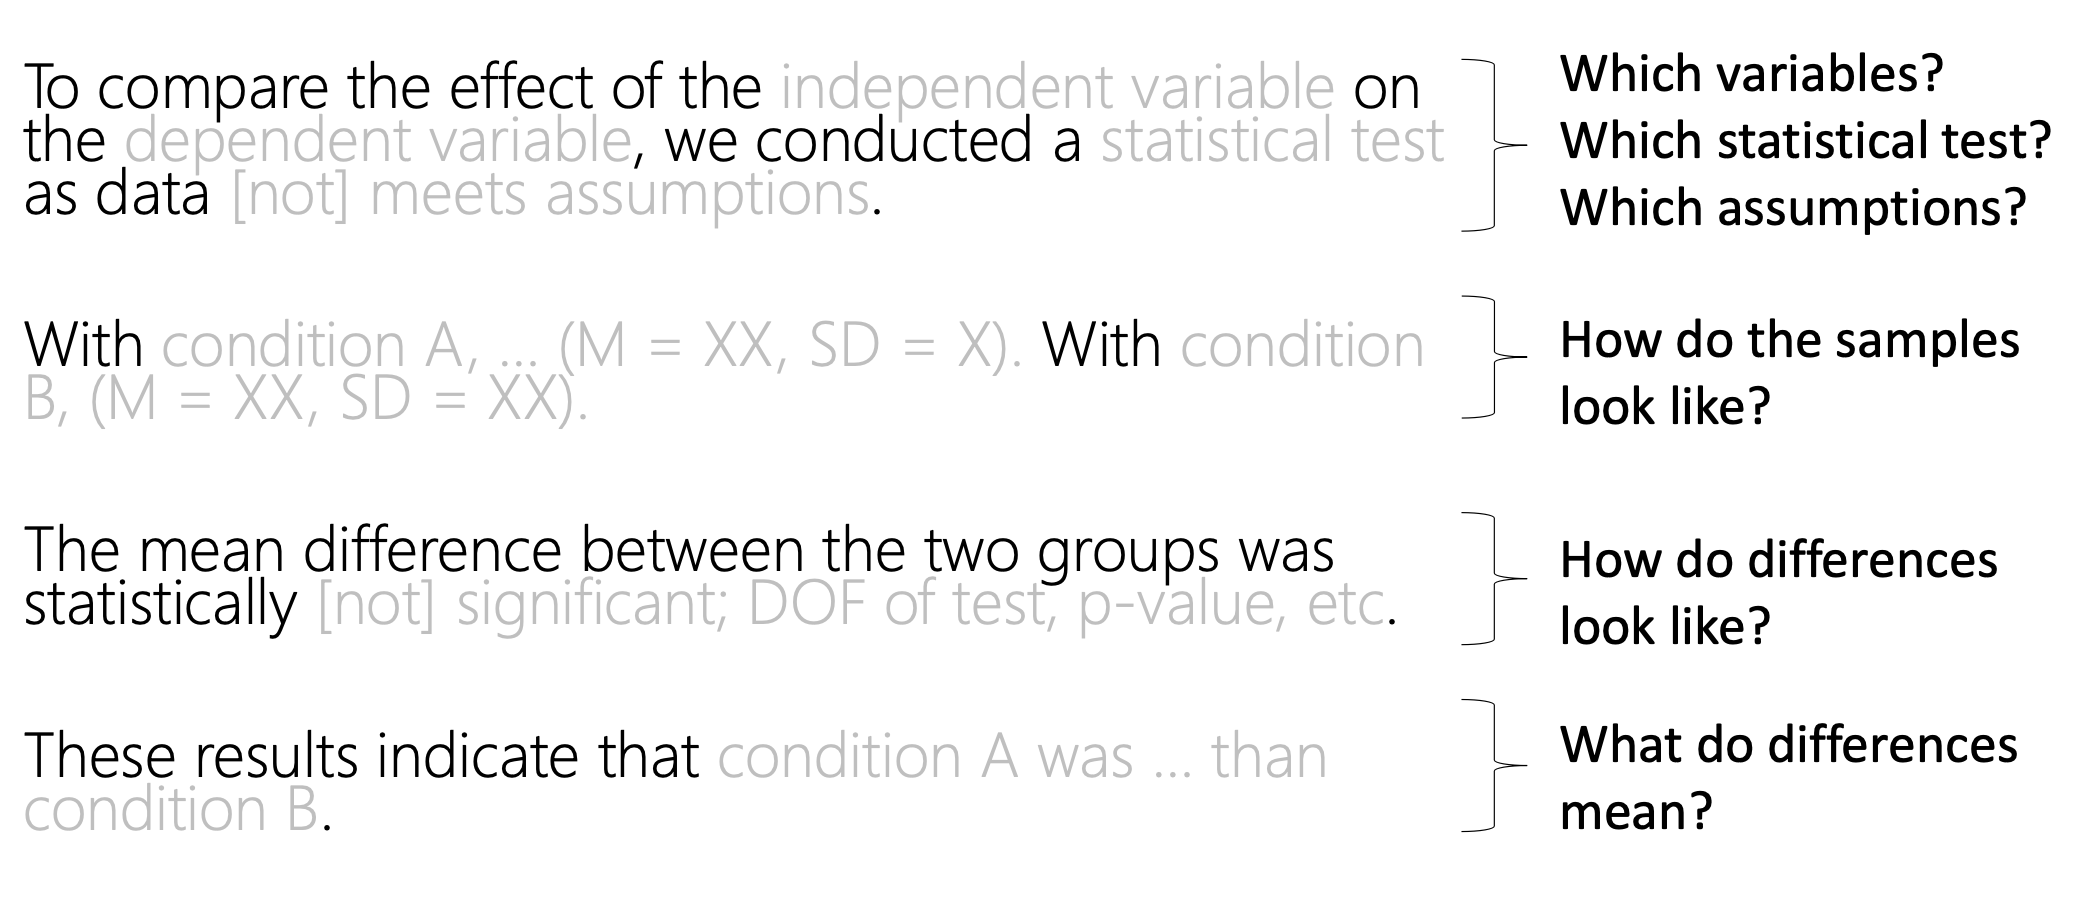
\includegraphics[width=\linewidth]{reporting.png}
\end{center}













